\documentclass[11pt,fleqn,twoside]{article}
\usepackage{makeidx}
\makeindex
\usepackage{palatino} %or {times} etc
\usepackage{plain} %bibliography style 
\usepackage{amsmath} %math fonts - just in case
\usepackage{amsfonts} %math fonts
\usepackage{amssymb} %math fonts
\usepackage{lastpage} %for footer page numbers
\usepackage{fancyhdr} %header and footer package
\usepackage{mmpv2} 
\usepackage{url}
\usepackage{float}
\usepackage{longtable}

% the following packages are used for citations - You only need to include one. 
%
% Use the cite package if you are using the numeric style (e.g. IEEEannot). 
% Use the natbib package if you are using the author-date style (e.g. authordate2annot). 
% Only use one of these and comment out the other one. 
\usepackage{cite}
\usepackage[parfill]{parskip}
%\usepackage{natbib}

\begin{document}

\name{Aidan Wynne Fewster}
\userid{awf1}
\projecttitle{NHS Wales formulary and antimicrobial Android application}
\projecttitlememoir{NHS Wales Android application} %same as the project title or abridged version for page header
\reporttitle{Requirements Specification}
\version{1.1}
\docstatus{Release}
\modulecode{CS39440}
\degreeschemecode{G400}
\degreeschemename{Computer Science}
\supervisor{Andrew Starr} % e.g. Neil Taylor
\supervisorid{aos}
\wordcount{}

%optional - comment out next line to use current date for the document
%\documentdate{10th February 2014} 
\mmp

\setcounter{tocdepth}{3} %set required number of level in table of contents


%==============================================================================
\section{Introduction}
%==============================================================================
\subsection{Purpose of this document}
%==============================================================================\
This document will outline the functional, user interface and security requirements for the NHS Wales formulary and antimicrobial Android application. It will also include use cases for the system. This document can later be used during testing to ensure that the system meets all the requirements outlined within.


%==============================================================================
\subsection{Project overview}
%==============================================================================
The main focus of this project is to produce a mobile application for Android which will aid NHS medical staff in obtaining useful information for injectable medicines which are available within the NHS . For more information refer to the Outline Specification document.


%==============================================================================
\section{Project details}
%==============================================================================
This section will describe the general factors that affect the requirements. It will describe the characteristics of the users using the system and explain how they shall be using the system. I will also outline any assumptions that I have made.

%==============================================================================
\subsection{User characteristics}
%==============================================================================
The primary users of the application will be medical staff of NHS Wales. They will be using the applications to search for information on drugs available within the NHS. They should already have broad knowledge of information displayed within the application. 

As the application will be built on the Android platform the member of staff should already be familiar with the user interface of Android and therefore be able to natively use applications that follow the Android design guidelines.

%==============================================================================
\subsection{Assumptions}
%==============================================================================
As the application will be used in hospitals I am assuming that an internet connection will not be available at all times when the application is in use therefore the data used by the application must be stored for offline use.

Another assumption I am making is that the member of staff will be installing the application on a device they are familiar with and therefore know how to use the basics of the Android operating system.

%==============================================================================
\subsection{Dependencies}
%==============================================================================
The application must have access to the NHS database in order to download the data required for the application. This access is provided via an XML API with a basic HTTP GET authentication procress (username and password are sent within the URL). All data transfered to and from the API is sent over HTTP without encryption (personally I would use an encypted connection for security reasons, but when asking the NHS about the secuirty of the data they said that secuirty was not a concern of theirs).


%==============================================================================
\section{Requirements}
%==============================================================================
\subsection{Functional requirements}
%==============================================================================
This section will list the functional requirement's (FR)'s for this project.

\begin{center}
\begin{longtable}{| l | p{14.3cm} |}
\hline
\textbf{FR 1}   & \textbf{Authentication}   \\ \hline
\textbf{FR 1.1} & User must be able to authenticate themselves using their credentials   \\ \hline
\textbf{FR 1.2} & User must be notified if the password they enter is incorrect\\ \hline
\textbf{FR 1.3} & User will be notified if the authentication failed due to connection issues \\ \hline
\textbf{FR 1.4} & User must be able to logout of the system, removing all data \\ \hline
\textbf{}  &  \\ \hline
\textbf{FR 2}   & \textbf{Database synchronisation}   \\ \hline
\textbf{FR 2.1} & After login or when the user presses update the application must truncate all database tables and begin downloading new data  \\ \hline
\textbf{FR 2.2} & Download complete list of drug indexes from database    \\ \hline
\textbf{FR 2.3} & Download complete list of drugs and drug information’s  \\ \hline
\textbf{FR 2.3} & Download all information needed for calculating doses and infusion rates.   \\ \hline
\textbf{FR 2.4} & Download must still run when the application is in the background \\ \hline
\textbf{}  &  \\ \hline
\textbf{FR 3}   & \textbf{Menu options}\\ \hline
\textbf{FR 3.1} & Upon pressing the Menu button on the device the user will be presented with a list of available options, which execute tasks (Logout, exit, search…)   \\ \hline
\textbf{}  &  \\ \hline
\textbf{FR 4}   & \textbf{Main screen} \\ \hline
\textbf{FR 4.1} & Upon successful data download the user will be displayed with a screen where they can navigate to other parts of the application   \\ \hline
\textbf{FR 4.2} & User will be see when an update was last performed, and perform an update from this screen.\\ \hline
\textbf{}  &  \\ \hline
\textbf{FR 5}   & \textbf{Browse drugs}\\ \hline
\textbf{FR 5.1} & This screen will allow the user to view a list of all drugs  \\ \hline
\textbf{FR 5.2} & There will be an input box on this screen, when the user enters text into the input box the results in the list will be filtered to only show results related to the input \\ \hline
\textbf{FR 5.3} & The user will be able to click a drug in the list to open a new screen displaying the needed information  \\ \hline
\textbf{}  &  \\ \hline
\textbf{FR 6}   & \textbf{View drug}   \\ \hline
\textbf{FR 6.1} & When a drug has been selected the drug and all it’s information will be displayed in an easy to read format    \\ \hline
\textbf{FR 6.2} & Where drug information headers contain help information, a help icon will be displayed next to the header.\\ \hline
\textbf{FR 6.3} & When heading help icon is clicked the helping information will be displayed \\ \hline
\textbf{FR 6.4} & If the drug had calculator information, then a button to open the calculator should be shown    \\ \hline
\textbf{}  &  \\ \hline
\textbf{FR 7}   & \textbf{Browse drugs with calculators}   \\ \hline
\textbf{FR 7.1} & A view similar to the browse drugs view will allow the browsing of drugs that contain calculator information.  \\ \hline
\textbf{}  &  \\ \hline
\textbf{FR 8}   & \textbf{Calculate dose and infusion rate}\\ \hline
\textbf{FR 8.1} & The user will be able to select calculation type   \\ \hline
\textbf{FR 8.2} & User will be able to enter information required for the calculation    \\ \hline
\textbf{FR 8.3} & When the calculate button has been clicked the input will be thoroughly validated\\ \hline
\textbf{FR 8.4} & After validation the result of the calculation will be displayed to the user\\ \hline
\textbf{FR 8.5} & The equation and values used to calculate the answer will be neatly displayed to the user  \\ \hline
\textbf{}  &  \\ \hline
\textbf{FR 9}   & \textbf{XML customisability – for developers} \\ \hline
\textbf{FR 9.1} & All text within the application must be changeable through XML files.  \\ \hline
\textbf{FR 9.2} & The structure of the XML API’s provided must be outline within XML files, allowing easy customisation for different API’s   \\ \hline
\end{longtable}
\end{center}


%==============================================================================
\subsection{User interface requirements}
%==============================================================================
The user interface for the application should follow the guidelines set out in the Android developer design guide. Following these guidelines will allow the user to learn to use the application with minimalistic effort.

When the user first opens the application, they will be presented with a login field. Upon logging in they will be presented with the latest updates to drugs and buttons. The buttons will allow the user to begin searching for a drug, force an update of the database and open the settings panel.

When the user selects a drug they will be presented with a neatly presented page with collapsible sections of information. This page will also contain a button to open the dosage calculation.

The user interface must be simplistic but make it clear what action you are currently performing. For example when calculating the dosage of penicillin for a patient, the user must be able to clearly see that penicillin has been selected and the weight of the patient used to calculate the dosage.
%==============================================================================
\subsection{Security}
%==============================================================================

The NHS have expressed concerns over the security of the data provided by the database. A number of problems will arise for the NHS should the information contained within the database be released to the public. It Is therefore fundamentally important that all data store on the device and all data transmitted to the device be encrypted.

The data stored on the device should be encrypted so that other applications can not access the information and should the device be placed in the hands of a malicious user the data should be inaccessible.

When database synchronisation occurs the data being transmitted should be transmitted over SSL so that the data is encrypted.


%==============================================================================
\section{Use case diagram}
%==============================================================================
\begin{figure}[H]
\centering
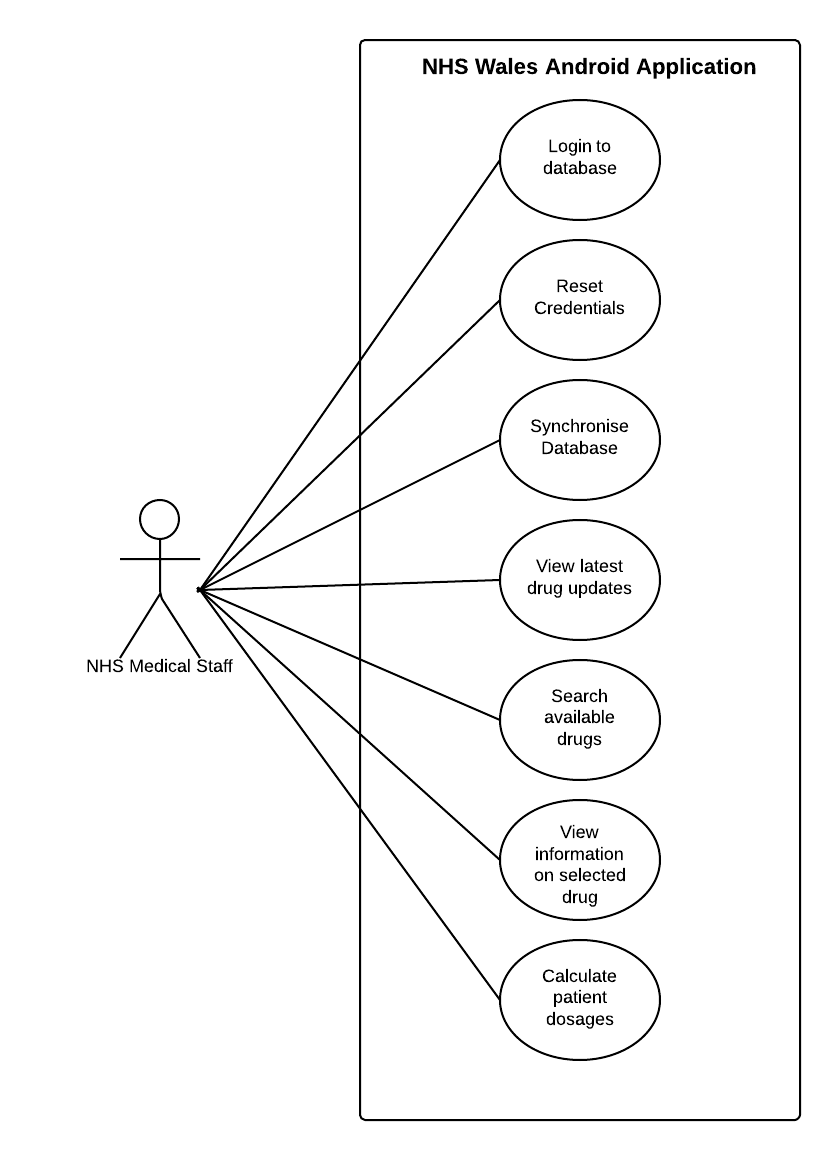
\includegraphics[width=4.4in]{useCase}
\caption{Use case diagram for the NHS application}
\end{figure}

\end{document}
